\documentclass[user_manual.tex]{subfiles}
\begin{document}
 \chapter{Primeros pasos}
 Antes de poner en funcionamiento a Justina, debemos conocer los software con los que trabaja y los requerimientos para  su correcto funcionamiento. También debes saber que Justina no funciona únicamente con una computadora, trabaja con 2 actualmente; en un computadora tenemos integrado ubuntu 14.04.1 (esta es la version ya probada), esta es la computadora principal, la cual se encargara de todos los procesos principales de Justina, y tenemos la seguna computadora con windows 7, la cual únicamente utilizaremos para la comunicación el reconocimiento por voz y el habla de Justina\\
 \\
 Como primer paso debemos conocer el software necesario para el funcionamiento de Justina.
 
 \section{Software necesario}

Se requiere lo siguiente:\\
\\
-Ubuntu
\begin{itemize}
\item ROS Indigo desktop full
\item OpenNI + PrimeSense drivers
\item OpenCV 2.4.8 or 2.4.9. Compiled with OpenNi, WITHOUT OpenCL, WITHOUT Cuda, with Eigen
\item PCL 1.6
\end{itemize}

Para conocer la forma de instalar ROS, OpenNI, los drivers PrimeSense y OpenCV 2.4.9 por favor acude al apéndice B (software).\\
\\
-Windows 7
\begin{itemize}
\item Blackboard
\item SpRecV1
\item SpRecV2
\end{itemize}

La comunicacion entre las dos computadoras se da por medio de conexion ethernet, para esto se debe configurar una computadora para que sea detectada como red. Para conocer la configuración de la red por favor visite el apendice de software.

 \section{Obtención de la carpeta de Git hub}
 Como siguiente paso obtener el software de Justina, para esto debemos descargar todas las carpetas con las que se ha 
 trabajado Justina.\\
 \\
 Todos los repositorios del software de Justina se encuentran en Git hub (así como este manual y es de donde podrás descargar futuras versiones). Existen dos formas para obtener la carpeta contenedora con todo lo necesario para empezar:\\
 \\
 La primera es ir a la dirección ``https://github.com/RobotJustina/JUSTINA/tree/develop`` y descargarlo con el botón color verde
 que dice "clone or download".\\
 \\
 \begin{center}
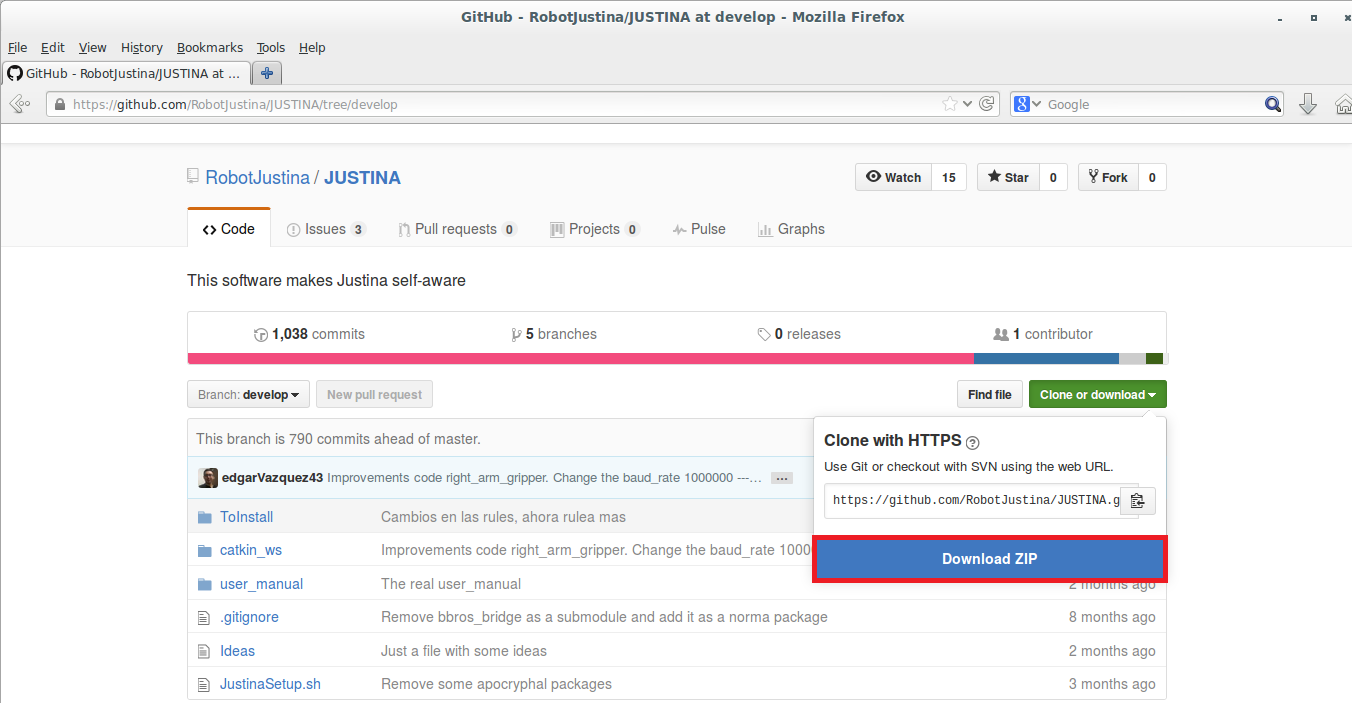
\includegraphics[width=0.85\textwidth]{Figures/PP/pp1.png}
\end{center}
\newpage
 te saldrá una opción para seleccionar la ubicación en la que deseas guardar el archivo .zip\\
 \\
 \begin{center}
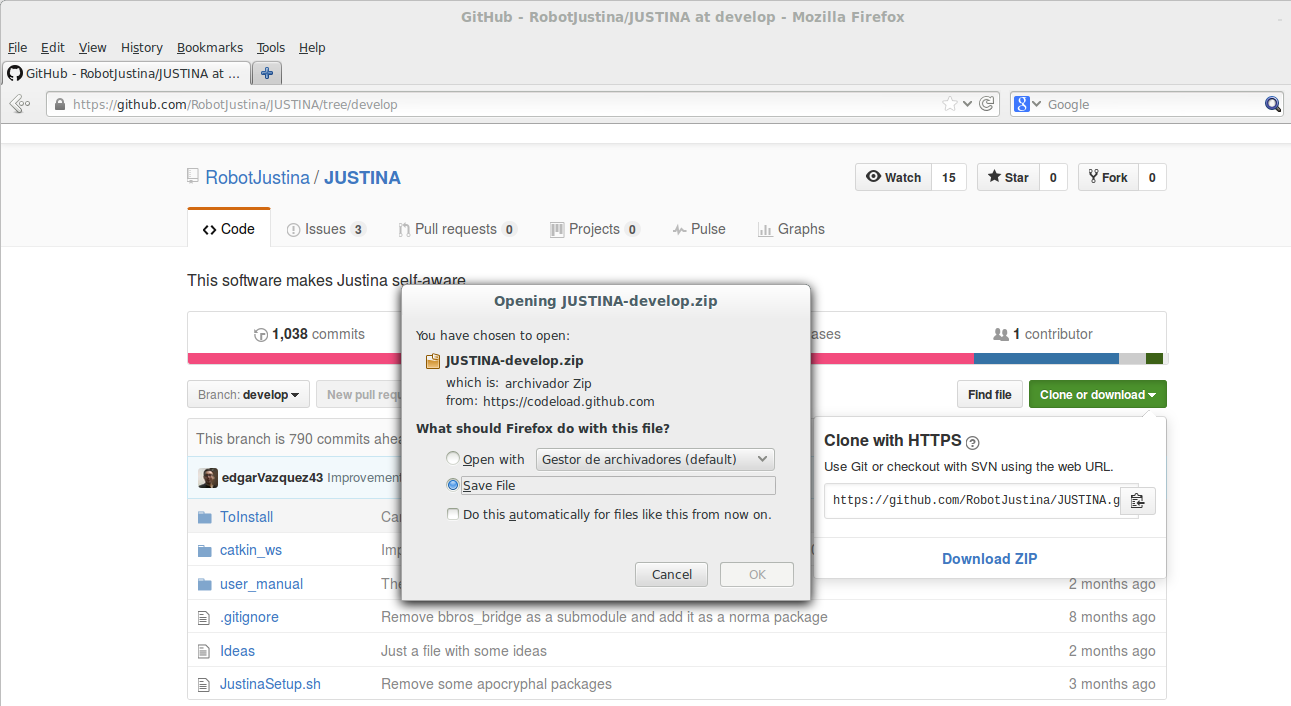
\includegraphics[width=0.8\textwidth]{Figures/PP/pp2.png}
\end{center}

 Busca la carpeta contenedora y descomprime el archivo. Al descomprimirlo obtendrás una carpeta llamada "JUSTINA" la 
 cual contiene todo lo necesario para utilizar a Justina.
 
 La segunda opción consiste  en que de desde la terminal clones la carpeta de Justina, usado el siguiente comando: ''git clone https://github.com/RobotJustina/JUSTINA``.
 
\section{Instalación del software de Justina}
Una vez instalado ROS procedemos a instalar el software de Justina, para esto abrir una terminal y seguir las siguientes instrucciones.

\begin{enumerate}
 \item ingresamos a la carpeta JUSTINA y ejecutar JustinaSetup.sh
  \begin{center}
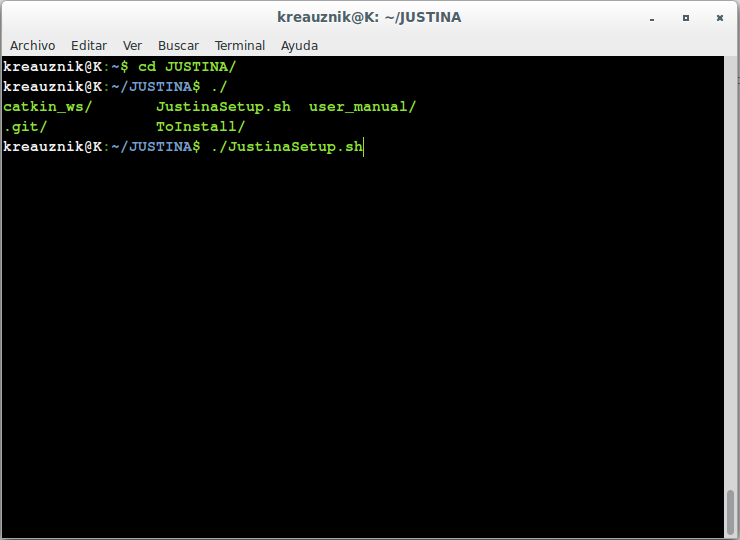
\includegraphics[width=0.73\textwidth]{Figures/PP/pp4.png}
\end{center}
 \item Aceptar cada que pregunte. Esto nos llevara varios minutos.
 \item Una vez instalado el software, debemos habilitar el uso de los puertos USB para ROS, para esto ingresamos al directorio "JUSTINA/ToInstall
 /USB (si quieres seguir las instrucciones más detalladamente, en la misma dirección abrir el archivo ``instructions'') una vez dentro
 de la carpeta ejecutar el siguiente comando "sudo cp 80-justinaRobot.rules /etc/udev/rules.d/"
 \item Te pedirá la contraseña. Una vez termines de ejecutar el comando, se debe ejecutar el siguiente: ``sudo udevadm control --reload-rules \&\& sudo service udev restart \&\& sudo udevadm trigger''
\end{enumerate}
Listo, ya tienes instalado el software de Justina.

\section{Cómo compilar los repositorios de Justina}
Para compilar los repositorios de Justina simplemente ve al directorio " JUSTINA/catkin\_ws", en este directorio ejecutamos el siguiente
comando ''catkin\_make". Esto nos llevara varios minutos.\\
\\
Una vez compilados todos los repositorios ejecutar el siguiente comando dentro de la misma carpeta " source devel/setup.bash".
 \begin{center}
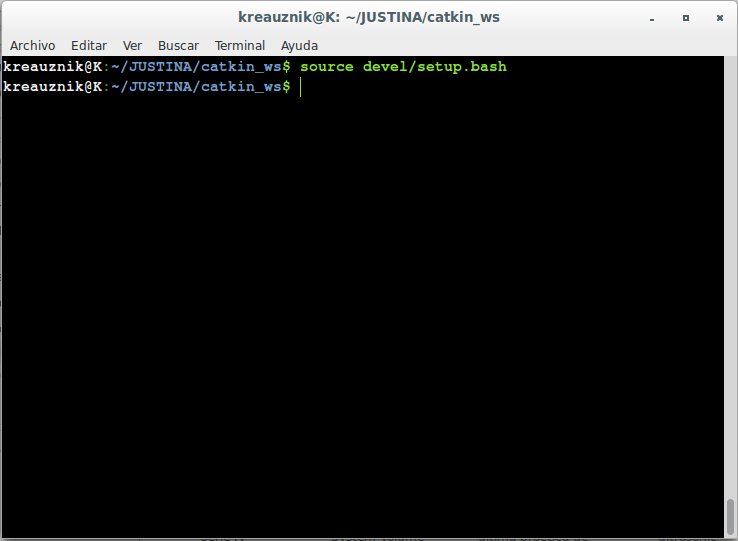
\includegraphics[width=0.73\textwidth]{Figures/PP/pp5.png}
\end{center}

Listo, ahora el software de Justina está instalado y los repositorios compilados y listos para usarse.

\section{RViz y GUI de Justina}
Para probar el funcionamiento del hardware y software de Justina utilizaremos RViz y la GUI. Para ejecutar estos programas utilizamos el 
comando ''roslaunch surge\_et\_ambula justina.launch".
 \begin{center}
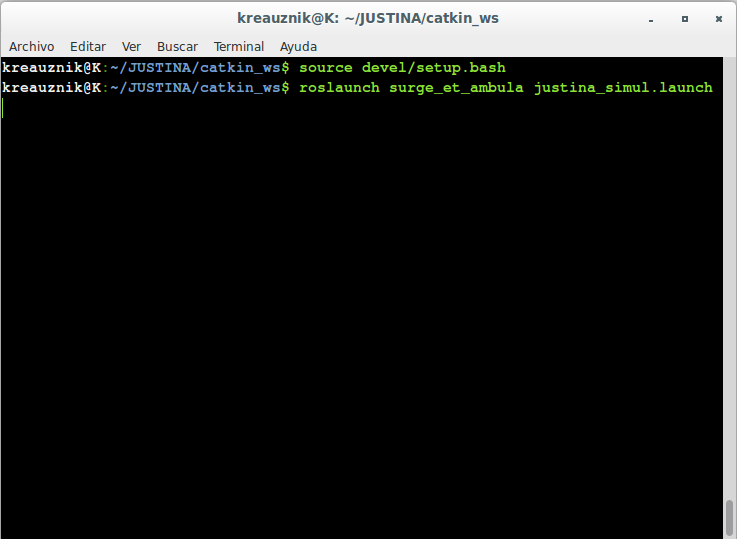
\includegraphics[width=0.73\textwidth]{Figures/PP/pp6.png}
\end{center}
\section{Simulación en el RViz y GUI de Justina}
Cuando no tenemos conectado el robot Justina a nuestras laptops lo único que podemos hacer
es simular a Justina en nuestras laptops, para esto ejecutamos el siguiente comando ''roslaunch surge\_et\_ambula justina\_simul.launch".




\end{document}
